\chapter*{Висновки}
\addcontentsline{toc}{chapter}{Висновки}

В результаті виконання роботи вдалося
\begin{enumerate}
  \item визначити оцінку (зглажування) часових рядів;
  \item зробити прогноз часових рядів на основі ретроданих;
  \item зробити прогноз часового ряду на основі моделі залежності
    від незалежних рядів.
\end{enumerate}

Хоча обидва методи показали себе добре,
проте прогноз на основі ретроданих краще.
Це було визначено за допомогою порівняння середньоквадратичного відхилення
помилок прогнозу для існуючих даних.
Прогноз за ретроданими дав помилку $\sigma = 24.06$,
а прогноз за прогнозами моделі $\sigma = 25.91$
(рис. \ref{fig:y:forecast:comparison}).
Це могло статися через ряд причин:
\begin{enumerate}
  \item кожен регресор мав свою похибку при прогнозі,
    потім ця похибка збільшилася при оцінці значення $Y$,
    коли оцінка $Y$ за ретроданими має лише свою похибку прогнозу;
  \item регресійна модель знайшла залежності, яких немає,
    але які допомагають покращити якість фільтрації,
    що також відомо як занадто точна регресія (overfitting);
    \cite{overfitting}
  \item обрано некоректні регресори;
  \item дані методи не підходять для цих даних.
\end{enumerate}

\begin{figure}[h!]
  \centering
  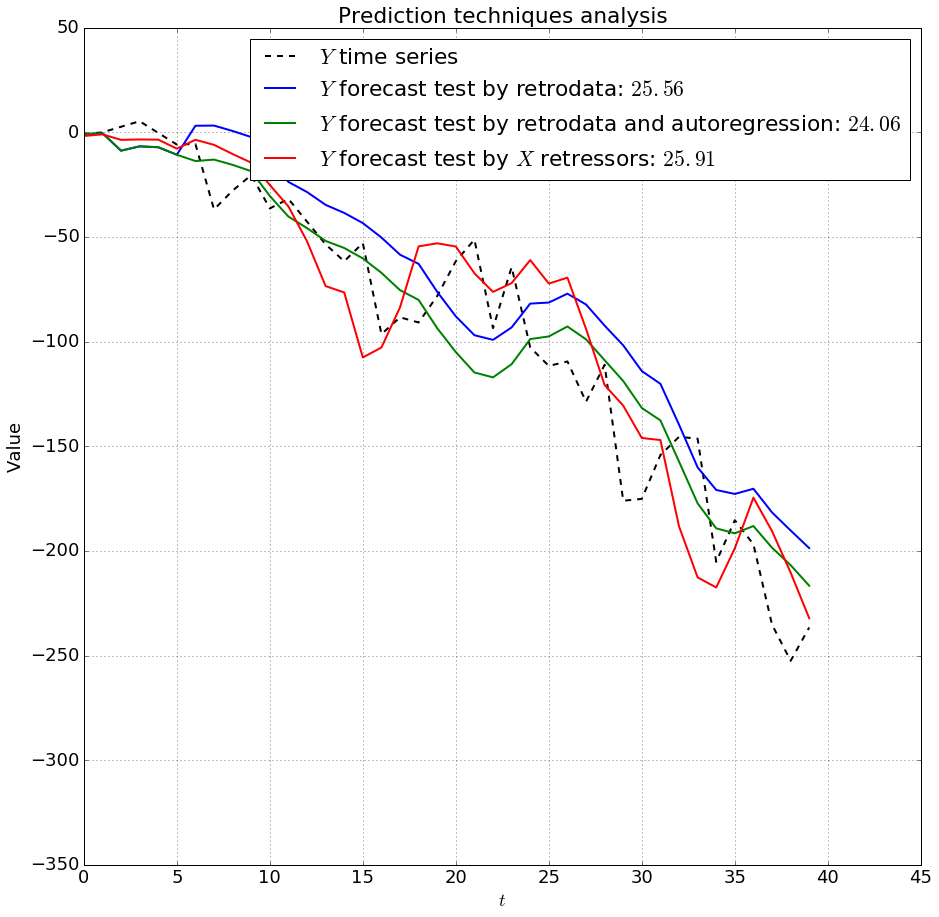
\includegraphics[width=\textwidth]{Coursework3_files/Coursework3_8_0.png}
  \caption{Порівняння прогнозів $Y$ за ретроданими та моделлю $X$}
  \label{fig:y:forecast:comparison}
\end{figure}
% \begin{center}
% \adjustimage{max size={0.9\linewidth}{0.9\paperheight}}{Coursework3_files/Coursework3_8_0.png}
% \end{center}
